\documentclass[../main.tex]{subfiles}
\begin{document}\label{chap3}

Với kiến thức tổng quan về PLS và CRN trình bày trong Chương \ref{chap2}, đặc biệt là các độ đo hiệu năng an toàn, trong chương này, bài toán cần giải quyết sẽ được mô tả cụ thể. Trước đó, mô hình hệ thống và mô hình tín hiệu sẽ được trình bày nhằm xác định cụ thể bối cảnh của bài toán, bao gồm các đối tượng trong hệ thống, thông tin mà các bên có và đặc điểm kênh truyền. Trên cơ sở đó, đồ án đề xuất hiệu năng đánh giá phù hợp và xây dựng bài toán tối ưu cho vấn đề thiết kế hệ thống.

\section{Mô hình hệ thống}

Đồ án này xem xét mô hình mạng vô tuyến nhận thức truy cập phổ đồng thời. Trong đó, tại bên sơ cấp, bên phát $\text{PTx}$ mong muốn truyền tin tới bên nhận $\text{PRx}$ đảm bảo an toàn bí mật trước một kẻ nghe lén thụ động $\text{EAVP}$. Tương tự, tại bên thứ cấp, bên phát $\text{STx}$ cũng cần truyền tin an toàn tới bên nhận $\text{SRx}$ trước nguy cơ nghe lén thụ động của $\text{EAVS}$, xem Hình~\ref{fig:SystemModel}. Đồ án này tập trung vào phân tích lợi ích của truyền tin hợp tác nên chỉ xem xét trường hợp các bên phát và thu tín hiệu đều chỉ trang bị một ăng-ten.

\begin{figure}
\centering
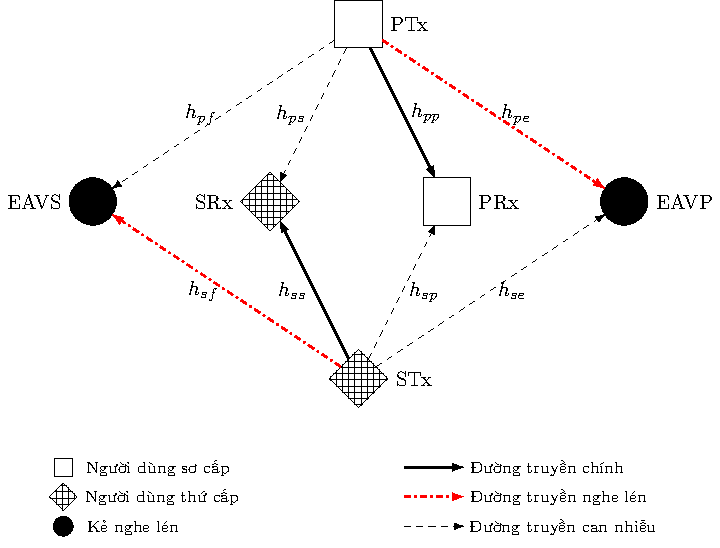
\includegraphics[width=0.9\linewidth]{model.pdf}
\caption{Mô hình hệ thống}
\label{fig:SystemModel}
\end{figure}

Trong mô hình này, $\text{PTx}$ và $\text{STx}$ có thể truyền tin đồng thời, trên cùng dải tần số được cấp quyền cho PU. Khi đó, tín hiệu nhận tại các bên thu có thể bao gồm can nhiễu từ các bên phát không mong muốn. Giả thiết rằng chiến lược giải mã của các bên thu sẽ coi tín hiệu không mong muốn là nhiễu và loại bỏ mà không giải mã.

Ngoài ra, như đã nói trong phần trước, có thể coi như các bên nhận và các bên nghe lén có đầy đủ CSI trên tất cả các kênh truyền từ các bên phát tới. Đối với CSIT, giả thiết rằng bên nhận không thực hiện phản hồi CSI về bên phát và kẻ nghe lén là thụ động nên CSI tại các bên phát là không hoàn hảo. Song, CSIT đóng vai trò quan trọng trong việc xác định chiến lược truyền an toàn nên coi các bên phát có được thông tin thống kê về các kênh truyền. Cụ thể, các bên phát có thể ước lượng được độ lợi kênh (channel gain) trung bình thông qua khoảng cách từ bên phát tới bên thu \cite{zou2010adaptive}.

Để đảm bảo an toàn bảo mật, các bên phát thực hiện chiến lược mã hóa ngẫu nhiên, trong đó mỗi thông điệp có thể được mã hóa thành nhiều từ mã \cite{wyner}. Tốc độ truyền từ mã $R_b$ và tốc độ truyền tin $R_s$ là hai tham số quan trọng phản ánh đặc điểm bộ mã hóa. Với mô hình đề xuất, các tham số này là cố định, điều này giúp giảm độ phức tạp của hệ thống, đồng thời phù hợp với một số ứng dụng đòi hỏi truyền tin với tốc độ cố định như truyền phát video \cite{he2016secrecy}.

\section{Mô hình tín hiệu}

Trong mô hình mạng vô truyến nhận thức truy cập phổ đồng thời, $\text{PTx}$ với tín hiệu $x_P^n=\left[x_P(1), x_P(2),..., x_P(n)\right]$ và $\text{STx}$ với tín hiệu $x_S^n=\left[x_S(1), x_S(2),..., x_S(n)\right]$ đồng thời truyền trên cùng một dải tần số, với $n$ là độ dài từ mã. Tốc độ truyền từ mã và tốc độ truyền tin đối với tín hiệu từ PU là $R_b^{(P)}$ và ${R_s^{(P)}}$, đối với SU là $R_b^{(S)}$ và ${R_s^{(S)}}$. Khi đó, tín hiệu nhận tại $\text{PRx}$ và $\text{SRx}$ tại thời điểm $i$ là:
\begin{align*}
y_P(i) = h_{pp}(i)x_P(i) + h_{sp}(i)x_S(i) + n_P(i), \\
y_S(i) = h_{ss}(i)x_S(i) + h_{ps}(i)x_P(i) + n_S(i),
\end{align*}
trong đó, $h_{pp}(i), h_{ps}(i), h_{ss}(i), h_{sp}(i)$ tương ứng là hệ số các kênh truyền $\text{PTx}\rightarrow\text{PRx}$, $\text{PTx}\rightarrow\text{SRx}$, $\text{STx}\rightarrow\text{SRx}$ và $\text{STx}\rightarrow\text{PRx}$; $n_P(i)$, $n_S(i)$ tương ứng là nhiễu Gauss trắng có tính cộng (additive white Gaussian noise - AWGN) tại $\text{PRx}$ và $\text{SRx}$, với trung bình là không và mật độ phổ công suất (power spectral density - PSD) tương ứng là $N_P$ và $N_S$.

Tương tự, tín hiệu nhận được tại $\text{EAVP}$ $y_E$ và tại $\text{EAVS}$ $y_F$ tương ứng là:
\begin{align*}
y_E(i) = h_{pe}(i)x_P(i) + h_{se}(i)x_S(i) + n_E(i), \\
y_F(i) = h_{sf}(i)x_S(i) + h_{pf}(i)x_P(i) + n_F(i),
\end{align*}
với $h_{pe}(i), h_{pf}(i), h_{se}(i), h_{sf}(i)$ tương ứng là hệ số các kênh truyền $\text{PTx}\rightarrow\text{EAVP}$, $\text{PTx}\rightarrow\text{EAVS}$, $\text{STx}\rightarrow\text{EAVP}$ và $\text{STx}\rightarrow\text{EAVS}$; $n_E(i)$, $n_F(i)$ tương ứng là nhiễu Gauss phức trắng có tính cộng tại $\text{EAVP}$ và $\text{EAVS}$, với trung bình không và mật độ phổ công suất tương ứng là $N_E$ và $N_F$.

Gọi các độ lợi kênh truyền trên là $g(i) = \left|h(i)\right|^2$, với $h(i)$ là hệ số kênh và bỏ qua việc thể hiện các chỉ số dưới nhằm chỉ chung cho tất cả các kênh truyền đã đề cập. Coi như tất cả các kênh truyền trong mô hình là kênh truyền suy hao Rayleigh bán tĩnh (quasi-static Rayleigh fading), tức là các độ lợi kênh truyền là không đổi trong suốt quá trình truyền từ mã và chúng là các biến ngẫu nhiên có phân phối mũ, với hàm mật độ xác suất (PDF) và hàm phân phối tích lũy (CDF) tương ứng là:
\begin{subequations}\label{channel}
\begin{align}
    f_X(x) &= \frac{1}{\Omega_X}\exp\left(-\frac{x}{\Omega_X}\right), \label{pdfc} \\
    F_X(x) &= 1-\exp\left(-\frac{x}{\Omega_X}\right), \label{cdfc}
\end{align}
\end{subequations}
trong đó, biến ngẫu nhiên $X$ đại diện cho độ lợi kênh truyền và $\Omega_X = \mathbb{E}\left\{X\right\}$ là trung bình độ lợi kênh tương ứng.

Ngoài ra các bên phát cũng bị giới hạn về năng lượng công suất phát, tức là:
\begin{subequations}\label{power}
\begin{align}
    p_P &= \frac{1}{n}\sum_{i=1}^{n}\left|x_P(i)\right|^2 \leq p_P^\text{max}, \label{pp} \\
    p_S &= \frac{1}{n}\sum_{i=1}^{n}\left|x_S(i)\right|^2 \leq p_S^\text{max}. \label{ps}
\end{align}
\end{subequations}

Thông qua tín hiệu mà các bên thu được, có thể xác định tỷ số tín hiệu trên nhiễu và can nhiễu (signal-to-interference-plus-noise ratio - SINR), từ đó xác định dung lượng kênh tức thời tại các bên nhận như sau:
\begin{subequations}\label{capacity}
\begin{align}
    C^{(P)} &= \log_2\left(1 + \text{SINR}^{(P)}\right) = \log_2\left(1 + \frac{p_Pg_{pp}}{p_Sg_{sp} + N_P}\right), \label{cp} \\
    C^{(E)} &= \log_2\left(1 + \text{SINR}^{(E)}\right) = \log_2\left(1 + \frac{p_Pg_{pe}}{p_Sg_{se} + N_E}\right), \label{ce} \\
    C^{(S)} &= \log_2\left(1 + \text{SINR}^{(S)}\right) = \log_2\left(1 + \frac{p_Sg_{ss}}{p_Pg_{ps} + N_S}\right), \label{cs} \\
    C^{(F)} &= \log_2\left(1 + \text{SINR}^{(F)}\right) = \log_2\left(1 + \frac{p_Sg_{sf}}{p_Pg_{pf} + N_F}\right), \label{cf}
\end{align}
\end{subequations}
trong đó các chỉ số trên $P, E, S, F$ lần lượt đại diện cho các bên nhận $\text{PRx}$, $\text{EAVP}$, $\text{SRx}$ và $\text{EAVS}$.

\section{Lựa chọn hiệu năng cho bài toán}

Mục tiêu của đồ án là thiết kế chiến lược truyền đảm bảo an toàn cho cả PU và SU. Do đó, một độ đo đánh giá mức độ an toàn là cần thiết cho bài toán thiết kế. Trong điều kiện chỉ có được các thông tin thống kê về kênh truyền, khi mà các bên phát không có đủ thông tin để lựa chọn chiến lược truyền luôn đảm bảo an toàn, các độ đo dựa trên xác suất mất an toàn thường được sử dụng để đánh giá hiệu năng. Song các độ đo này không phản ánh định lượng lượng thông tin bị nghe lén khi sự kiện mất an toàn xảy ra. Do đó, trong đồ án này, tốc độ lộ tin trung bình (AILR) sẽ được sử dụng là mục tiêu cho bài toán thiết kế.

Như đã đề cập, tốc độ truyền từ mã $R_b^{(P)}$ và ${R_b^{(S)}}$ trong mô hình là không đổi, trong khi, dưới ảnh hưởng của suy hao, dung lượng tức thời trên các kênh truyền chính $C^{(P)}, C^{(S)}$ có thể thấp hơn tốc độ này, dẫn đến giải mã sai ở các bên nhận mong muốn. Do đó, để đảm bảo truyền tin tin cậy, giả thiết rằng các bên nhận $\text{PRx}$ và $\text{SRx}$ đều có một kênh phản hồi tới bên phát tương ứng. Tương tự trong \cite{zhou2011, he2016secrecy}, các bên nhận, với kết quả ước lượng dung lượng kênh của mình, có thể phản hồi một bit tới bên phát để đảm bảo bên phát chỉ truyền thông điệp khi $R_b^{(P)} \leq C^{(P)}$ và $R_b^{(S)} \leq C^{(S)}$. Với chiến lược này, xác suất truyền tương ứng là:
\begin{subequations}\label{ptx}
\begin{align}
    p_{tx}^{(P)} &= \mathbb{P}\left(R_b^{(P)} \leq C^{(P)}\right), \label{ptxp} \\
    p_{tx}^{(S)} &= \mathbb{P}\left(R_b^{(S)} \leq C^{(S)}\right). \label{ptxs}
\end{align}
\end{subequations}

Tác giả trong \cite{he2016secrecy} đã chứng minh rằng: với điều kiện $R_b^{(P)} \leq C^{(P)}$ và $R_s^{(P)} \leq R_b^{(P)}$, mức độ không rõ ràng $\Delta$ \eqref{delta} tại kẻ nghe lén $\text{EAVP}$ với dung lượng kênh $C^{(E)}$ có thể viết lại thành:
\begin{equation}\label{deltap}
\Delta^{(P)}=
\begin{cases}
1,& \text{nếu } C^{(E)}\leq R_b^{(P)} - R_s^{(P)}\\
\left(R_b^{(P)} - C^{(E)}\right)/R_s^{(P)},& \text{nếu } R_b^{(P)} - R_s^{(P)} < C^{(E)} < R_b^{(P)}\\
0 ,& \text{nếu } R_b^{(P)} \leq C^{(E)},
\end{cases}
\end{equation}

Từ đó, tốc độ lộ tin trung bình tại PU với tốc độ truyền tin $R_s^{(P)}$ cố định là:
\begin{equation}\label{rlp}
R_L^{(P)} = \left(1-{\Bar{\Delta}}^{(P)}\right)R_s^{(P)},
\end{equation}
và độ đo hiệu năng GSOP là:
\begin{align}\label{gsopp}
p_{out}^{(P)}\left(\delta^{(P)}\right) = \mathbb{P}\left(\Delta^{(P)} < \delta^{(P)}\right).
\end{align}

Các công thức $\Delta^{(S)}$, $R_L^{(S)}$, $p_{out}^{(S)}$ ứng với SU và kẻ nghe lén $\text{EAVS}$ được phát biểu tương tự.

\begin{equation}\label{deltas}
\Delta^{(S)}=
\begin{cases}
1,& \text{nếu } C^{(F)}\leq R_b^{(S)} - R_s^{(S)}\\
\left(R_b^{(S)} - C^{(F)}\right)/R_s^{(S)},& \text{nếu } R_b^{(S)} - R_s^{(S)} < C^{(F)} < R_b^{(S)}\\
0 ,& \text{nếu } R_b^{(S)} \leq C^{(F)},
\end{cases}
\end{equation}

\begin{equation}\label{rls}
R_L^{(S)} = \left(1-{\Bar{\Delta}}^{(S)}\right)R_s^{(S)},
\end{equation}

\begin{align}\label{gsops}
p_{out}^{(S)}\left(\delta^{(S)}\right) = \mathbb{P}\left(\Delta^{(S)} < \delta^{(S)}\right).
\end{align}

\section{Phát biểu bài toán}

Đồ án này thực hiện giải quyết bài toán an toàn bảo mật cho mô hình trên theo hướng tiếp cận cấp phát công suất truyền cho các bên PTx và STx, đảm bảo truyền thông tin cậy và an toàn cho cả hai bên. Cụ thể, dựa trên độ đo an toàn bảo mật AILR và độ đo về chất lượng truyền tin là xác suất truyền tin, bài toán thiết kế trên được mô hình qua một bài toán tối ưu đa mục tiêu:
\begin{subequations}\label{moop}
\begin{align}
\underset{p_P, p_S}{\text{minimize}} \quad & R_{L}^{(P)}, R_{L}^{(S)} \nonumber \\
\text{s.t} 
\quad & p_{tx}^{(P)} \geq \sigma^{(P)}, \label{moop:ptxp}\\
\quad & p_{tx}^{(S)} \geq \sigma^{(S)}, \label{moop:ptxs}\\
\quad & 0 \leq p_P \leq p_P^\text{max}, \label{moop:pp}\\
\quad & 0 \leq p_S \leq p_S^\text{max}, \label{moop:ps}
\end{align}
\end{subequations}
trong đó $\sigma^{(P)}, \sigma^{(S)} \in [0, 1]$ là xác suất truyền tối thiểu mà các bên yêu cầu đạt được; $p_P^\text{max}, p_S^\text{max}$ là công suất phát tối đa mà các bên phát có thể dùng. Khi xem xét điều kiện ràng buộc về công suất phát tối đa tại SU \eqref{moop:ps} và xác suất truyền của PU \eqref{moop:ptxp}, bài toán tối ưu này cũng phản ánh điều kiện cần để SU có thể sử dụng chiến lược truy cập phổ đồng thời để truyền tin cùng với PU, đó là yêu cầu công suất phát của SU không làm giảm chất lượng truyền tin của PU \cite{tran2017cognitive,quach2017secrecy}.

Trong mô hình CRN truyền thống, việc chia sẻ tài nguyên tần số thường không mang lại lợi ích cho PU, thậm chí can nhiễu từ SU có thể gây suy giảm chất lượng truyền tin tại PU. Tuy nhiên, khi xét thêm yếu tố an toàn, can nhiễu từ SU có thể làm suy giảm chất lượng tín hiệu nghe lén của $\text{EAVP}$ nhiều hơn đáng kể so với suy giảm gây ra cho $\text{PRx}$. Song, kết quả này cũng phụ thuộc vào các điều kiện kênh truyền từ $\text{STx}$ tới $\text{PRx}$ và $\text{EAVP}$. Do đó, PU hoàn toàn có thể lựa chọn chia sẻ tài nguyên tần số và cùng truyền với SU chỉ khi việc hợp tác này giúp cải thiện chất lượng truyền tin an toàn tại PU. Như vậy, một cách tự nhiên, bài toán thiết kế chiến lược truyền này cần dành cho SU giải quyết. Khi đó, SU có thể tùy chỉnh các tham số của bài toán để cân bằng giữa lợi ích từ việc được truyền tin (bằng việc gia tăng hiệu năng an toàn cho PU) và chất lượng truyền tin an toàn của chính mình.

Trong mô hình này, SU sẽ thực hiện giải bài toán thiết kế \eqref{moop} nên giả thiết rằng PU và SU có thể truyền thông với nhau, tức là có một kênh truyền kết nối PU và SU \cite{su2012active}. Qua đó các bên có thể thống nhất các tham số cần thiết, đồng thời SU sau khi giải quyết bài toán tối ưu, có thể đề xuất chiến lược truyền tới PU và PU cũng có thể thông báo về quyết định hợp tác của mình.

\section{Kết chương}

Qua việc xây dựng mô hình và đưa ra các giả thiết về kênh truyền, CSI tại các bên và chiến lược mã hóa, chương này đã cụ thể hóa bài toán thiết kế hệ thống dưới dạng một bài toán tối ưu đa mục tiêu. Cách thức giải quyết bài toán này sẽ được đề cập trong chương sau.

\end{document}